\documentclass[conference]{IEEEtran}

\usepackage[utf8]{inputenc}
\usepackage[T1]{fontenc}
\usepackage[spanish,es-nodecimaldot,es-noshorthands]{babel}
\usepackage{amsmath,amssymb}
\usepackage{graphicx}
\usepackage{booktabs}
\usepackage{array}
\usepackage{xcolor}
\usepackage{url}
\usepackage{cite}
\usepackage{tikz}
\usetikzlibrary{positioning,arrows.meta,calc}

\graphicspath{{figuras/}}

% Marca de datos por completar (quitar cuando se llenen)
\newcommand{\pend}[1]{\textcolor{red}{[#1]}}

\begin{document}

\title{IMPLEMENTACIÓN EXPERIMENTAL DE UN ENLACE BFSK PARA TELEMETRÍA INDUSTRIAL CON USRP 2920 Y HACKRF ONE EN GNU RADIO}

\author{
\IEEEauthorblockN{Edward Andres Pacheco Jurado- 2222236, Angely Yulitza Vásquez Lozada- 2222240\\
Daniel Eduardo Suarez Jaimes- 2222228}
\IEEEauthorblockA{Universidad Industrial de Santander\\
Escuela de Ingenierías Eléctrica, Electrónica y de Telecomunicaciones\\
GitHub: \url{https://github.com/EDWARDPJ26/2026_2_CommII_A1_GA1D_PRoYECTO_FINAL}}
}

\maketitle

\begin{abstract}
This work presents the experimental implementation of the binary frequency shift keying (BFSK) link designed in the previous phases for an industrial telemetry application. The simulated channel was replaced by a physical over-the-air link at 870~MHz, using an NI USRP 2920 as transmitter (UHD: USRP Sink) and a HackRF One as receiver (osmocom Source), both controlled from GNU Radio 3.10. The hardware parameters of each radio were identified and configured, and the relation between the baseband sample rate (1~MS/s) and the radio sample rate (1~MS/s in the USRP, 8~MS/s in the HackRF with decimation by 8) was established without modifying the symbol rate of 10~kbaud. Two controlled tests were performed at a distance of about 3~m: an ideal transmission and a transmission with injected AWGN ($\sigma = 0.6$). In both cases the spectrum analyzer measured a tone separation of 40.8~kHz, consistent with the designed deviation of $\pm 20$~kHz, and the receiver recovered the transmitted 16-bit pattern without visible errors.
\end{abstract}

\begin{IEEEkeywords}
BFSK, SDR, USRP 2920, HackRF One, UHD, gr-osmosdr, GNU Radio, telemetría industrial.
\end{IEEEkeywords}

\section{Introducción}

En las fases anteriores del proyecto el enlace BFSK para telemetría industrial se estudió completamente en simulación: se generó la modulación, se modeló el canal con ruido AWGN e interferencia y se diseñó un receptor capaz de recuperar la información~\cite{guia1,guia2}. El paso siguiente consiste en sustituir el canal simulado por un enlace físico usando radios definidos por software (SDR).

Esta fase no busca medir BER, sino reconocer y configurar correctamente las interfaces de hardware que conectan el transmisor y el receptor ya diseñados con los radios disponibles~\cite{guia3}: un NI USRP 2920 para transmitir y un HackRF One para recibir. El objetivo es documentar qué parámetros controla cada radio, cuáles dependen del modelo de hardware y cómo se relacionan con las variables de banda base de la simulación, sin alterar injustificadamente los parámetros de diseño de la aplicación.

\section{Metodología}

\subsection{Hardware y software}

El Cuadro~\ref{tab:hw} resume los equipos y el software utilizados. El transmisor y el receptor se ejecutaron en dos computadores distintos: el del USRP, que tiene los controladores UHD y la conexión Ethernet al equipo, y un portátil con el HackRF conectado por USB.

\begin{table}[!t]
\centering
\caption{Hardware y software empleados.}
\label{tab:hw}
\begin{tabular}{>{\raggedright}p{2.1cm}p{5.6cm}}
\toprule
Elemento & Descripción \\
\midrule
Transmisor & NI USRP 2920 (equivalente al Ettus N210), tarjeta WBX de 50~MHz a 2.2~GHz, ganancia TX de 0 a 31.5~dB, conexión Gigabit Ethernet. \\
Receptor & HackRF One: 1~MHz a 6~GHz, half-duplex, muestras I/Q de 8~bits, de 2 a 20~MS/s, conexión USB~2.0. \\
Antenas & Antenas del laboratorio, una en cada radio, con ancho de banda que cubre la frecuencia de trabajo de 870~MHz. \\
Verificación & Analizador de espectro. \\
Software & GNU Radio 3.10.12.0 (radioconda), UHD 4.8.0, gr-osmosdr y libhackrf 2024.02.1. \\
\bottomrule
\end{tabular}
\end{table}

\subsection{Del canal simulado al enlace físico}

Siguiendo la guía~\cite{guia3}, los flujogramas simulados se conservaron como referencia y se crearon copias específicas para hardware:
\begin{itemize}
\item \texttt{Transmisor\_FSK\_USRP\_Ruido.grc}: transmisor BFSK con la posibilidad de inyectar AWGN y un tono interferente antes del USRP.
\item \texttt{Receptor\_FSK\_HackRF\_Ojo.grc}: receptor digital alimentado por el HackRF, con espectros, frecuencia instantánea, diagrama de ojo y constelación I-Q.
\end{itemize}

En ambos archivos se eliminó el bloque \textit{Channel Model}, porque el canal ahora es el medio físico, y se eliminó el \textit{Throttle}, porque el ritmo de las muestras lo imponen el DAC del USRP y el ADC del HackRF. La Fig.~\ref{fig:enlace} muestra el enlace de prueba: se transmitió por aire a una distancia aproximada de 3~m, con el analizador de espectro como verificación independiente.

\begin{figure}[!t]
\centering
\resizebox{\columnwidth}{!}{%
\begin{tikzpicture}[
  blk/.style={draw, rounded corners, align=center, minimum height=1.0cm, font=\small},
  >={Latex[length=2mm]}]
\node[blk] (pc1) {PC Tx\\GNU Radio + UHD};
\node[blk, right=0.7cm of pc1] (usrp) {USRP 2920\\puerto TX/RX};
\node[blk, right=2.2cm of usrp] (hrf) {HackRF One\\puerto ANT};
\node[blk, right=0.7cm of hrf] (pc2) {PC Rx\\GNU Radio + osmosdr};
\node[blk, below=1.0cm of $(usrp)!0.5!(hrf)$] (an) {Analizador de\\espectro};
\draw[->] (pc1) -- node[above, font=\scriptsize]{Ethernet} (usrp);
\draw[->] (hrf) -- node[above, font=\scriptsize]{USB 2.0} (pc2);
\draw[->, dashed] (usrp) -- node[above, font=\scriptsize]{aire, $\approx$3~m} node[below, font=\scriptsize]{870~MHz} (hrf);
\draw[->, dashed] (usrp) -- (an);
\end{tikzpicture}}
\caption{Diagrama del enlace físico de prueba. Ambos radios usan antenas del laboratorio cuyo ancho de banda cubre los 870~MHz; no se usaron cables ni atenuadores, por lo que se trabajó con ganancias bajas en los dos extremos.}
\label{fig:enlace}
\end{figure}

\subsection{Transmisor con USRP 2920}

La Fig.~\ref{fig:flujotx} muestra el flujograma del transmisor. La secuencia de 16~bits \texttt{[0,1,0,0,1,1,0,1,1,1,0,0,1,0,1,0]} se repite de forma continua, se mapea a NRZ ($0 \rightarrow -1$, $1 \rightarrow +1$), se interpola por $sps = 100$ y modula en frecuencia con sensibilidad
\begin{equation}
k = \frac{2\pi \, \Delta f}{f_s} = \frac{2\pi \cdot 20\,\text{kHz}}{1\,\text{MS/s}} = 0.1257~\text{rad/muestra}.
\end{equation}
A la señal FSK de amplitud unitaria se le suman, de forma opcional, ruido gaussiano complejo de desviación $\sigma$ y un tono interferente de amplitud relativa $A$. El conjunto se escala con
\begin{equation}
\text{norm} = \frac{1}{1 + 3\sigma + A}
\end{equation}
para que el pico de la envolvente no supere 1 y el DAC no sature, sin cambiar la relación $E_b/N_0$ ni la SIR. La amplitud digital final es $\texttt{tx\_amp}\cdot\text{norm}$, con $\texttt{tx\_amp} = 0.7$.

\begin{figure*}[!t]
\centering
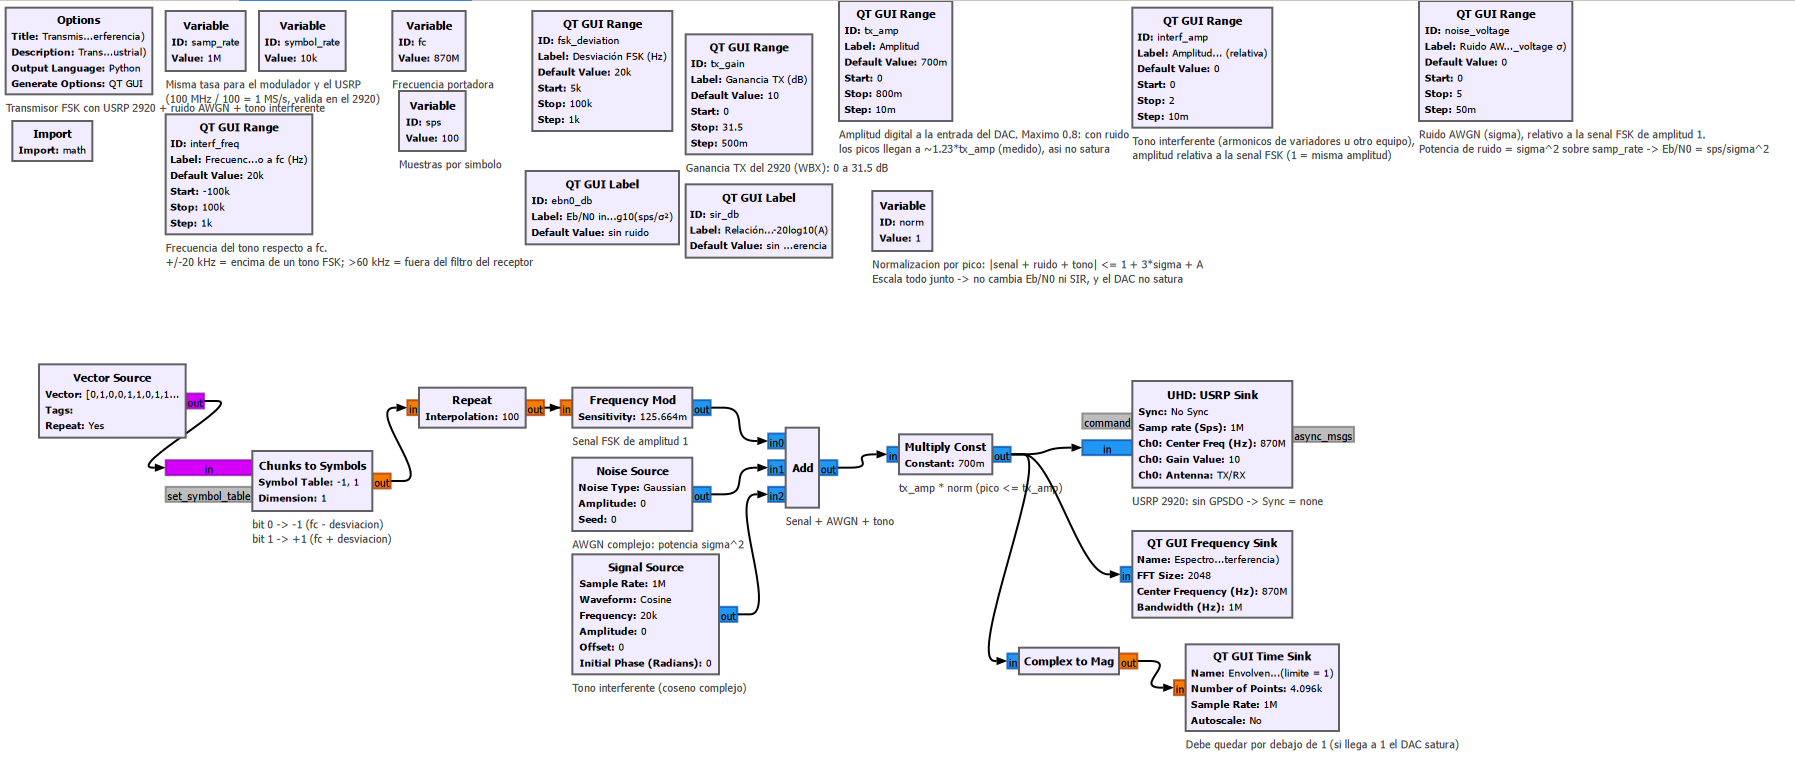
\includegraphics[width=\textwidth]{flujo_tx.png}
\caption{Flujograma del transmisor \texttt{Transmisor\_FSK\_USRP\_Ruido.grc}: Vector Source, mapeo NRZ, Repeat, Frequency Mod, suma de AWGN y tono interferente, normalización y UHD: USRP Sink. Incluye el espectro transmitido y la envolvente a la entrada del DAC.}
\label{fig:flujotx}
\end{figure*}

Las Figs.~\ref{fig:uhdgen} y~\ref{fig:uhdrf} muestran la configuración del bloque \textit{UHD: USRP Sink}, y el Cuadro~\ref{tab:uhd} explica cada parámetro~\cite{uhdsink,uhd}.

\begin{figure}[!t]
\centering
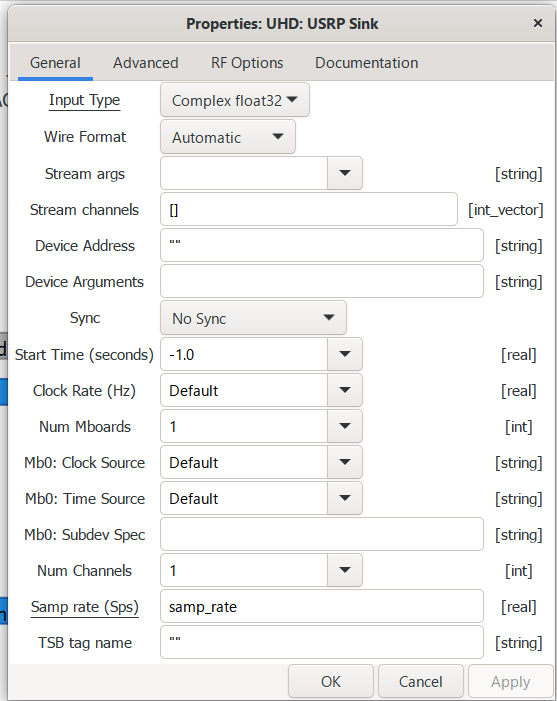
\includegraphics[width=0.8\columnwidth]{uhd_sink_general.png}
\caption{UHD: USRP Sink, pestaña \textit{General}.}
\label{fig:uhdgen}
\end{figure}

\begin{figure}[!t]
\centering
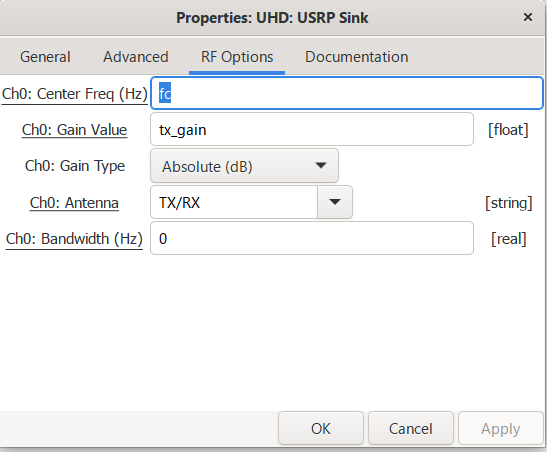
\includegraphics[width=0.8\columnwidth]{uhd_sink_rf.png}
\caption{UHD: USRP Sink, pestaña \textit{RF Options}.}
\label{fig:uhdrf}
\end{figure}

\begin{table}[!t]
\centering
\caption{Parámetros del bloque UHD: USRP Sink.}
\label{tab:uhd}
\begin{tabular}{>{\raggedright}p{1.9cm}>{\raggedright}p{1.5cm}p{4.1cm}}
\toprule
Parámetro & Valor & Justificación \\
\midrule
Device Address & \texttt{""} & UHD usa el primer USRP que encuentra. Con varios equipos se usaría \texttt{addr=<IP>} (el 2920 va por Ethernet) o \texttt{serial=<n>}. \\
Sync & No Sync & El 2920 no tiene GPSDO; con \texttt{gps\_time} el programa fallaba. \\
Clock/Time Source & Default & Reloj interno; no hay referencia externa de 10~MHz/PPS. \\
Num Channels & 1 & La WBX tiene un canal de TX. \\
Sample Rate & 1~MS/s & $100\,\text{MHz}/100$: tasa exacta para el reloj maestro del 2920. \\
Center Freq & 870~MHz & Frecuencia del proyecto, junto a la banda SRD de 863--870~MHz. \\
Gain & 20~dB & Rango de la WBX: 0--31.5~dB. Valor bajo por la cercanía de los radios. \\
Antenna & TX/RX & Único puerto que transmite (RX2 solo recibe). \\
Bandwidth & 0 (auto) & No configurable en la WBX; se deja automático. \\
Input Type & fc32 & Muestras complejas en punto flotante. \\
\bottomrule
\end{tabular}
\end{table}

\subsection{Receptor con HackRF One}

La Fig.~\ref{fig:flujorx} muestra el flujograma del receptor. El HackRF entrega 8~MS/s; el \textit{Frequency Xlating FIR Filter} recentra el canal ($f_{\text{centro}} = \texttt{lo\_offset} + \texttt{freq\_corr}$), filtra con un pasa bajas de 60~kHz y decima por 8 para volver a 1~MS/s. Después el \textit{Quadrature Demod} con ganancia $f_s/(2\pi\Delta f)$ entrega la frecuencia instantánea normalizada en $\pm 1$; el \textit{DC Blocker} elimina el desplazamiento residual causado por el error de frecuencia entre radios; un pasa bajas de 10~kHz limpia el ruido; y la cadena \textit{Delay} + \textit{Keep 1 in N} + \textit{Binary Slicer} toma una muestra por símbolo y decide el bit.

\begin{figure*}[!t]
\centering
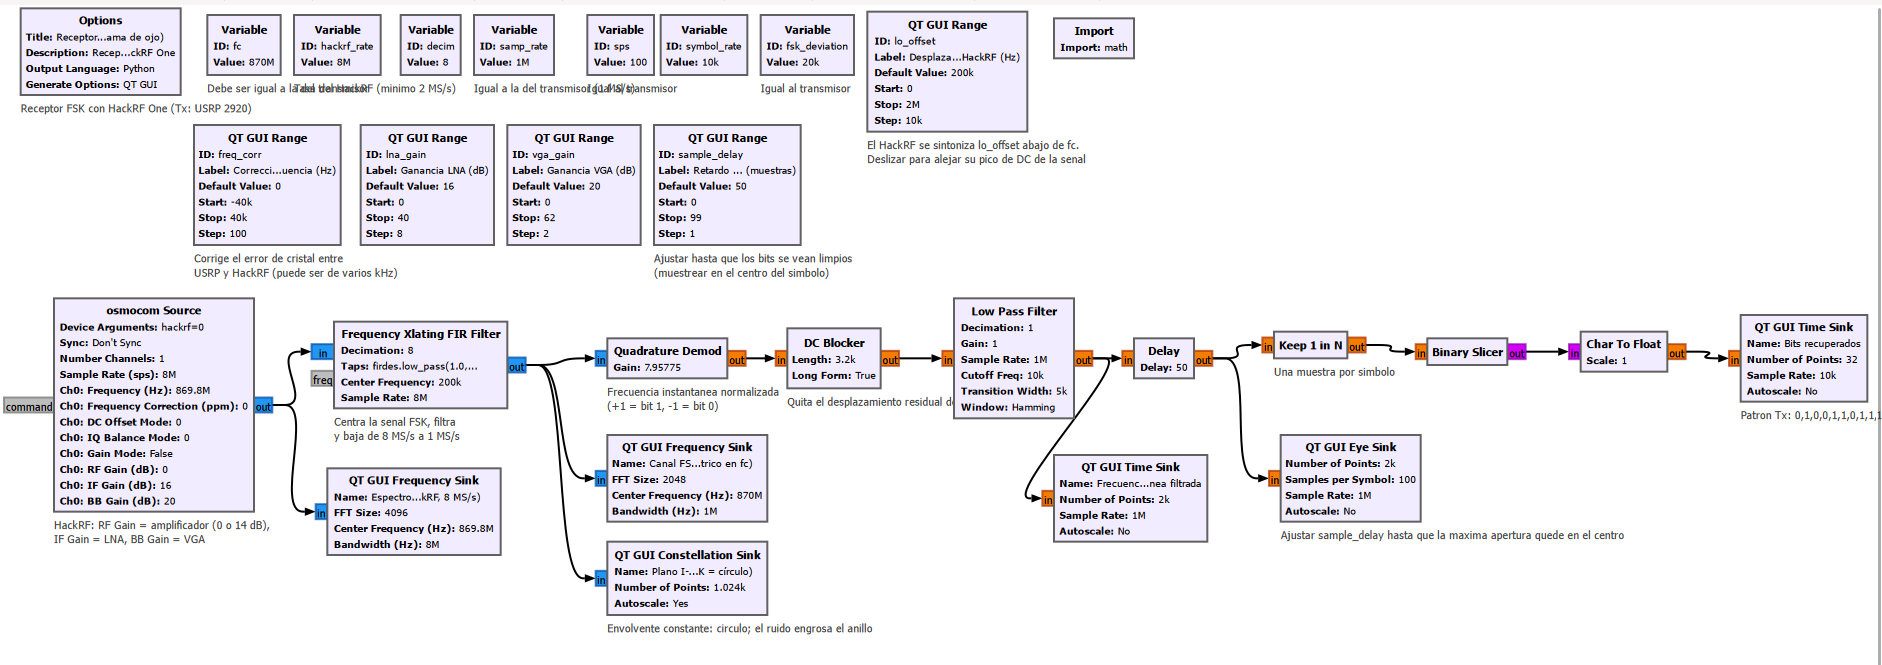
\includegraphics[width=\textwidth]{flujo_rx.png}
\caption{Flujograma del receptor \texttt{Receptor\_FSK\_HackRF\_Ojo.grc}: osmocom Source, Frequency Xlating FIR Filter (decimación 8), Quadrature Demod, DC Blocker, Low Pass Filter, Delay, Keep 1 in N y Binary Slicer, con espectros, frecuencia instantánea, diagrama de ojo, plano I-Q y bits recuperados.}
\label{fig:flujorx}
\end{figure*}

Respecto al receptor de la Fase~2, que usaba \texttt{Delay = 200} muestras, la versión de hardware agrega las etapas que solo aparecen con radios reales: la traslación y decimación desde la tasa del HackRF, la corrección de frecuencia \texttt{freq\_corr} y el \textit{DC Blocker}. El retardo de muestreo pasa a ser un control deslizante (\texttt{sample\_delay}), porque la latencia del enlace real no es fija.

La Fig.~\ref{fig:osmo} muestra la configuración del bloque \textit{osmocom Source}, y el Cuadro~\ref{tab:osmo} explica cada parámetro. En osmocom, para el HackRF, \textit{RF Gain} corresponde al amplificador interno (AMP, 0 o 14~dB), \textit{IF Gain} al LNA (0--40~dB en pasos de 8) y \textit{BB Gain} al VGA (0--62~dB en pasos de 2)~\cite{hackrf,osmosdr}.

\begin{figure}[!t]
\centering
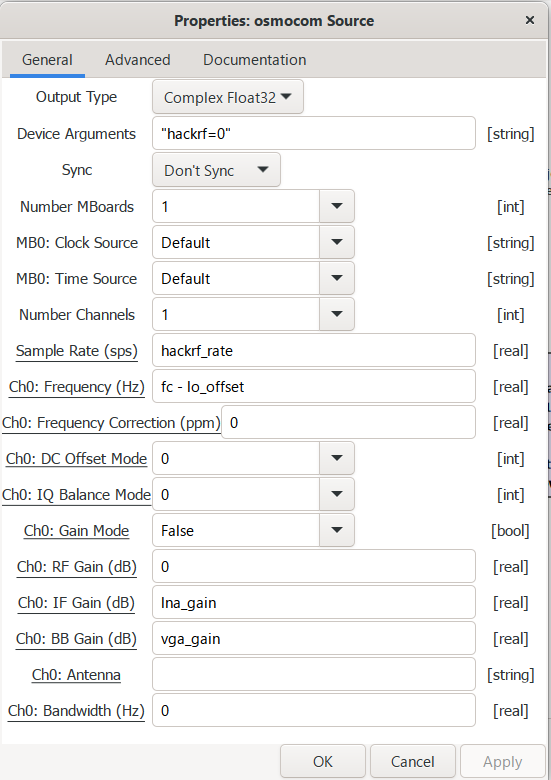
\includegraphics[width=0.8\columnwidth]{osmocom_general.png}
\caption{Configuración del bloque osmocom Source para el HackRF One.}
\label{fig:osmo}
\end{figure}

\begin{table}[!t]
\centering
\caption{Parámetros del bloque osmocom Source.}
\label{tab:osmo}
\begin{tabular}{>{\raggedright}p{1.9cm}>{\raggedright}p{1.5cm}p{4.1cm}}
\toprule
Parámetro & Valor & Justificación \\
\midrule
Device Arguments & \texttt{hackrf=0} & Primer HackRF conectado. Con varios equipos: \texttt{hackrf=<serial>}. \\
Sample Rate & 8~MS/s & El HackRF necesita al menos 2~MS/s; 8~MS/s es múltiplo entero de 1~MS/s. \\
Frequency & $f_c - \texttt{lo\_offset}$ & Permite desplazar la señal fuera del pico de DC del receptor. \\
Freq. Corr. (ppm) & 0 & La corrección se hace en Hz con \texttt{freq\_corr} en el Xlating FIR. \\
DC Offset / IQ Balance & 0 & Sin corrección automática; el DC se evita con \texttt{lo\_offset} y el DC Blocker. \\
Gain Mode & False & Sin AGC; ganancias manuales. \\
RF Gain (AMP) & 0~dB & Amplificador apagado: los radios están cerca. \\
IF Gain (LNA) & \texttt{lna\_gain} & Por defecto 16~dB. \\
BB Gain (VGA) & \texttt{vga\_gain} & Por defecto 20~dB. \\
Bandwidth & 0 (auto) & El HackRF elige su filtro de banda base según la tasa de muestreo. \\
Antenna & vacío & El HackRF tiene un solo puerto de antena. \\
Bias-T & no activado & No aparece como campo; se activaría con \texttt{bias=1} en Device Arguments. Alimentaría con 3.3~V un LNA externo, por lo que no debe activarse con una antena pasiva conectada. \\
\bottomrule
\end{tabular}
\end{table}

\subsection{Tasa de banda base frente a tasa del radio}

La tasa de banda base del diseño es
\begin{equation}
bb\_rate = R_s \cdot sps = 10\,\text{kbaud} \times 100 = 1~\text{MS/s}.
\end{equation}
En el transmisor, el USRP 2920 acepta exactamente esa tasa ($100\,\text{MHz}/100$), así que
\begin{equation}
radio\_rate_{\text{Tx}} = bb\_rate \times \frac{1}{1} = 1~\text{MS/s},
\end{equation}
sin remuestreo. En el receptor, el HackRF trabaja a 8~MS/s y se aplica la adaptación inversa antes del receptor digital:
\begin{equation}
bb\_rate = radio\_rate_{\text{Rx}} \times \frac{1}{8} = \frac{8~\text{MS/s}}{8} = 1~\text{MS/s}.
\end{equation}
La decimación la hace el propio \textit{Frequency Xlating FIR Filter}, que al mismo tiempo actúa como filtro anti-aliasing. $R_s$ \textbf{no cambió}: se mantuvo en 10~kbaud, el valor justificado por la aplicación de telemetría, y todos los bloques posteriores del receptor trabajan a la tasa de diseño de 1~MS/s.

\subsection{Procedimiento de prueba}

Se ejecutó primero el transmisor y después el receptor. Se realizaron dos pruebas controladas por aire, con $\texttt{tx\_gain} = 20$~dB, $\texttt{tx\_amp} = 0.7$ y $\Delta f = 20$~kHz:
\begin{itemize}
\item \textbf{Prueba 1:} transmisión ideal, $\sigma = 0$ y sin tono interferente.
\item \textbf{Prueba 2:} transmisión con AWGN inyectado, $\sigma = 0.6$, equivalente a un $E_b/N_0 = 10\log_{10}(sps/\sigma^2) = 24.4$~dB en el transmisor. El tono interferente se dejó apagado ($A = 0$).
\end{itemize}
En ambas pruebas se registraron el espectro transmitido, el espectro medido con el analizador y las gráficas del receptor. Los parámetros del transmisor se leen directamente en las capturas de sus controles (Figs.~\ref{fig:p1tx} y~\ref{fig:p2tx}). En el receptor se usaron los valores por defecto del flujograma (Fig.~\ref{fig:flujorx}): \texttt{freq\_corr} = 0, LNA = 16~dB, VGA = 20~dB, AMP apagado y \texttt{sample\_delay} = 50. La única excepción fue \texttt{lo\_offset}: el espectro recibido aparece centrado en 870~MHz, lo que indica que durante las pruebas se dejó en 0.

\section{Resultados}

\subsection{Prueba 1: transmisión ideal}

La Fig.~\ref{fig:p1tx} muestra el espectro generado en el transmisor: los dos lóbulos de la FSK en $f_c \pm 20$~kHz y una envolvente constante de 0.7 a la entrada del DAC, por debajo del límite de 1.

\begin{figure}[!t]
\centering
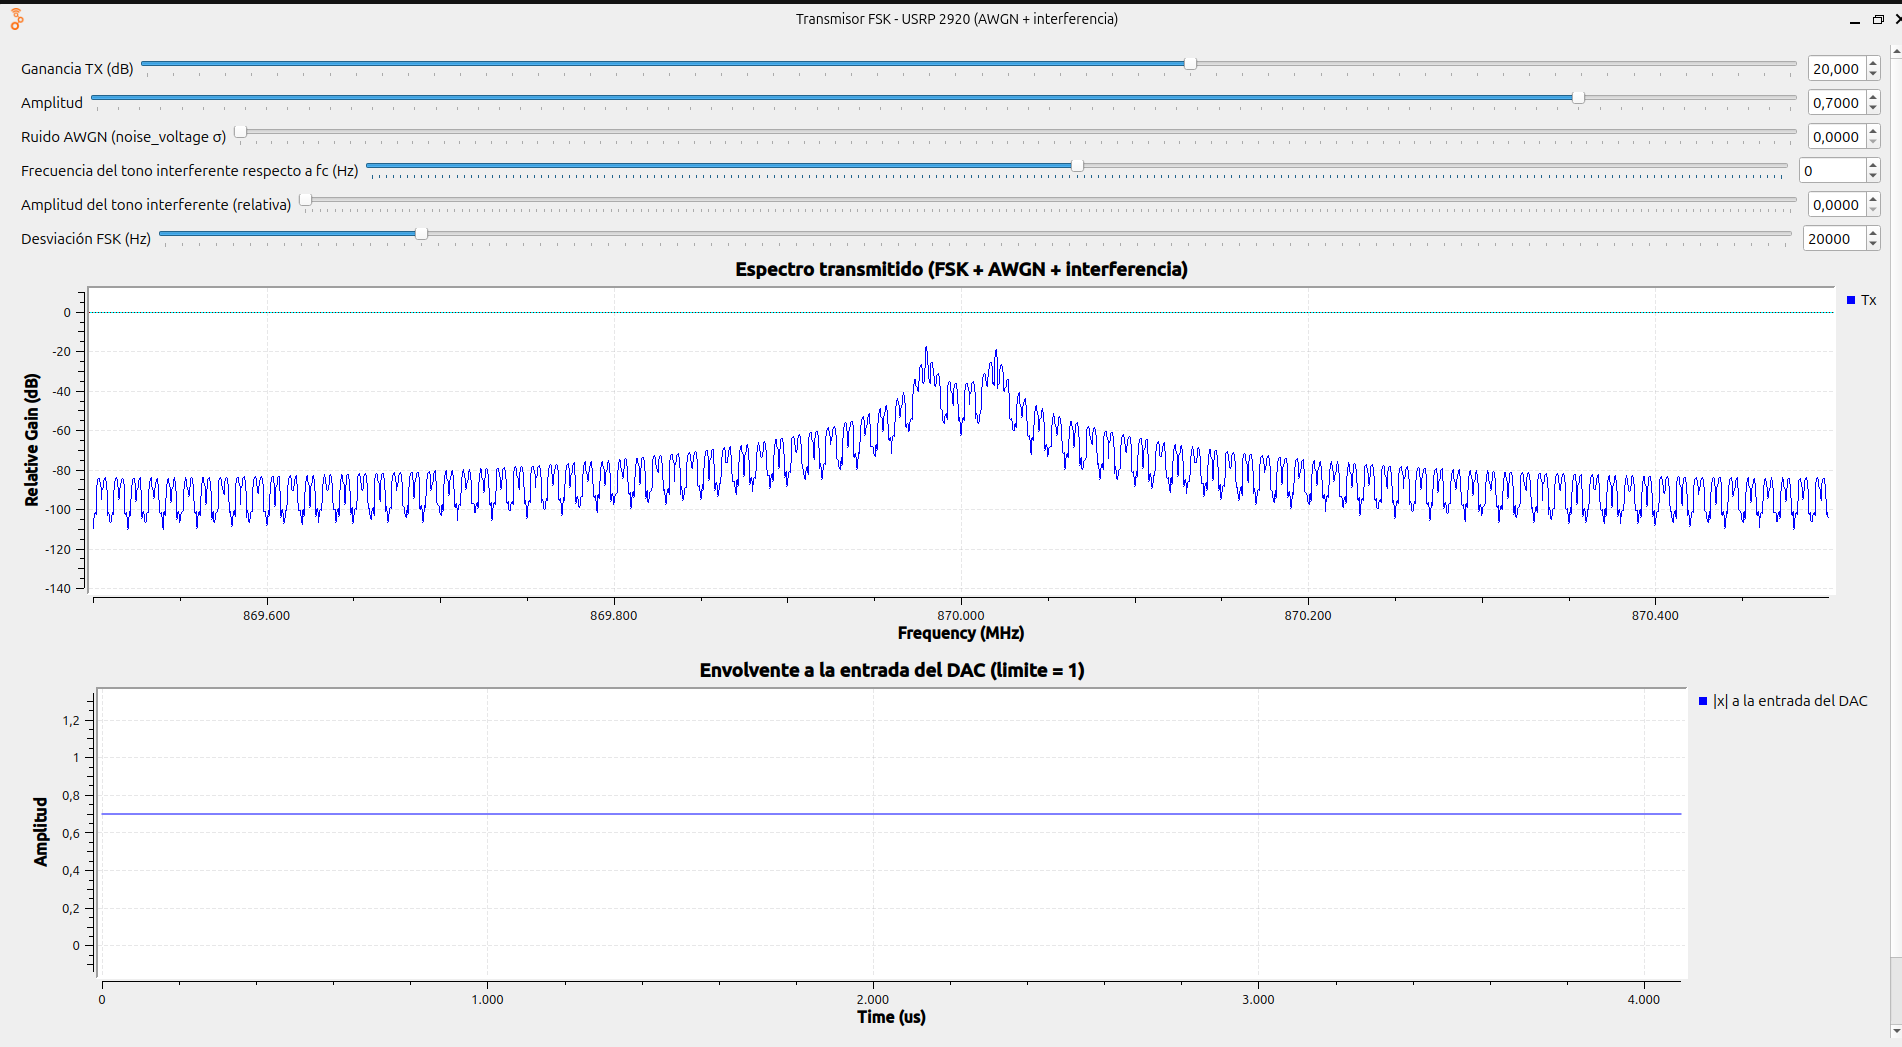
\includegraphics[width=\columnwidth]{p1_tx.png}
\caption{Prueba 1, transmisor: espectro transmitido y envolvente a la entrada del DAC ($\sigma = 0$, $\texttt{tx\_gain} = 20$~dB).}
\label{fig:p1tx}
\end{figure}

En el analizador de espectro (Fig.~\ref{fig:p1an}) el marcador M1 se ubica en 869.9787~MHz con $-45.18$~dBm, y el marcador delta D2 mide una separación de 40.801~kHz con 0.59~dB de diferencia entre tonos. La separación coincide con $2\Delta f = 40$~kHz dentro de la resolución del barrido (span de 1~MHz, RBW de 3~kHz), y el piso de ruido queda cerca de $-105$~dBm.

\begin{figure}[!t]
\centering
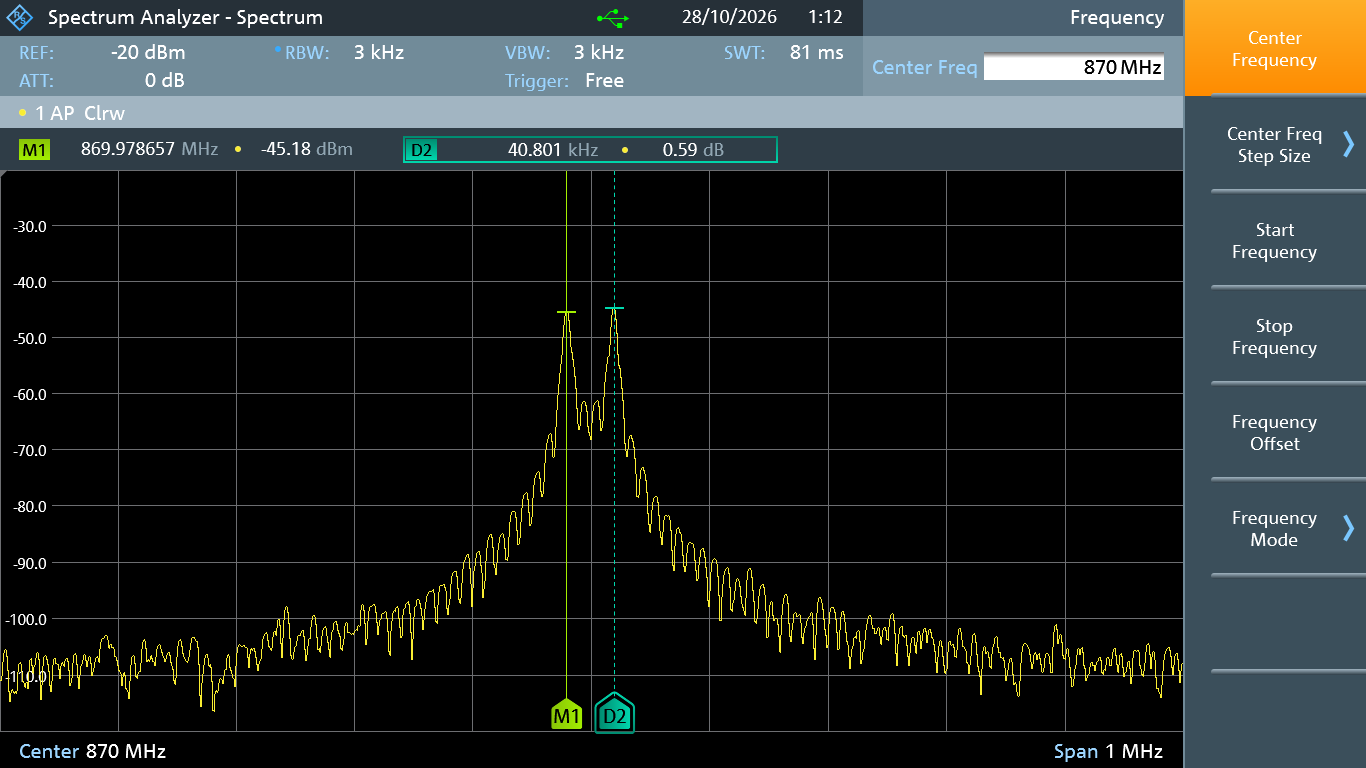
\includegraphics[width=\columnwidth]{p1_analizador.png}
\caption{Prueba 1, analizador de espectro: centro 870~MHz, span 1~MHz, RBW 3~kHz. Separación entre tonos de 40.801~kHz.}
\label{fig:p1an}
\end{figure}

En el receptor (Fig.~\ref{fig:p1rx}) la señal aparece en 870~MHz dentro de los 8~MHz que observa el HackRF, con un piso cerca de $-90$~dB relativos. El plano I-Q de la señal filtrada forma un anillo delgado, que es lo esperado para una modulación de envolvente constante. La frecuencia instantánea filtrada es una onda cuadrada entre $\pm 1$, el diagrama de ojo está completamente abierto y los bits recuperados forman la secuencia periódica \texttt{1001101110010100}, que es el patrón transmitido rotado un bit. La rotación es normal, porque el enlace no tiene sincronización de trama.

\begin{figure}[!t]
\centering
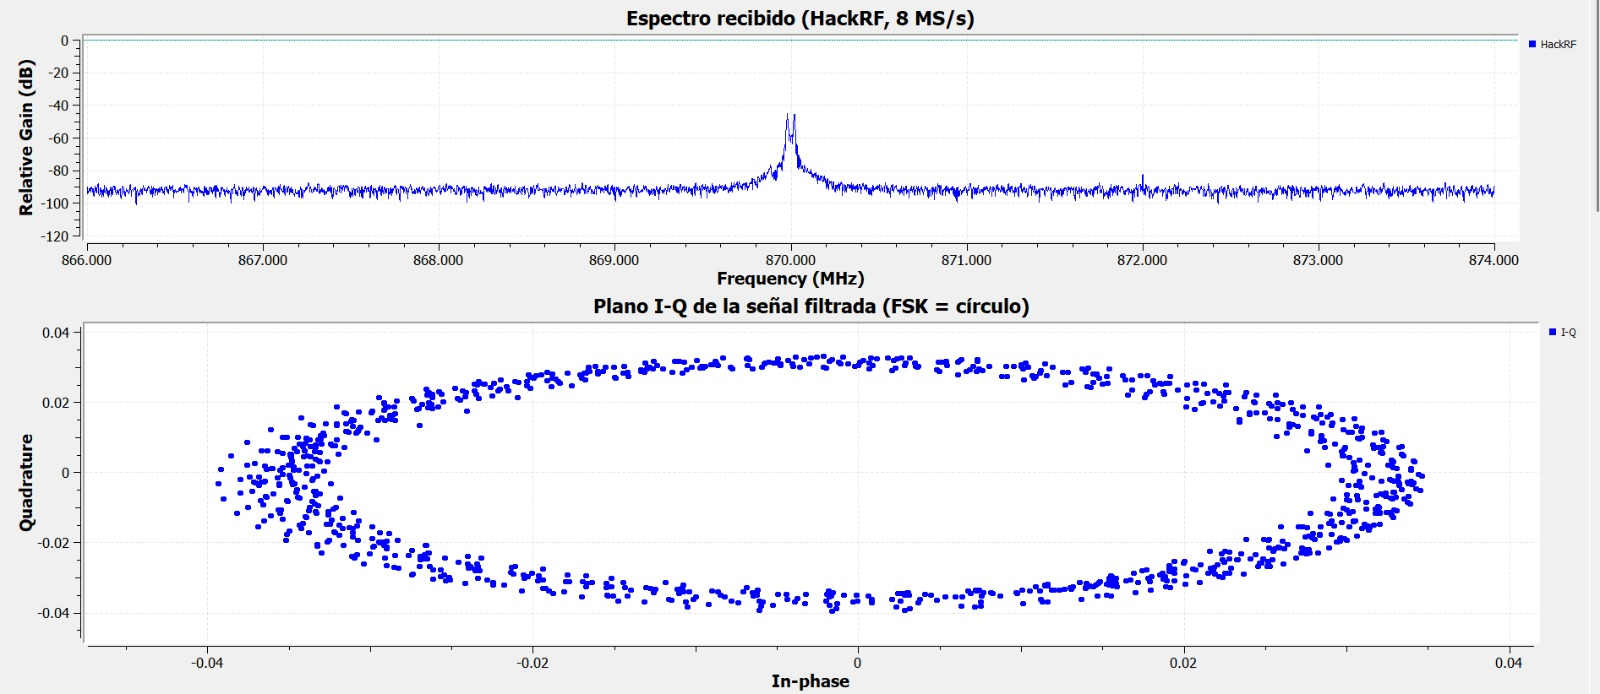
\includegraphics[width=\columnwidth]{p1_rx1.jpeg}\\[2pt]
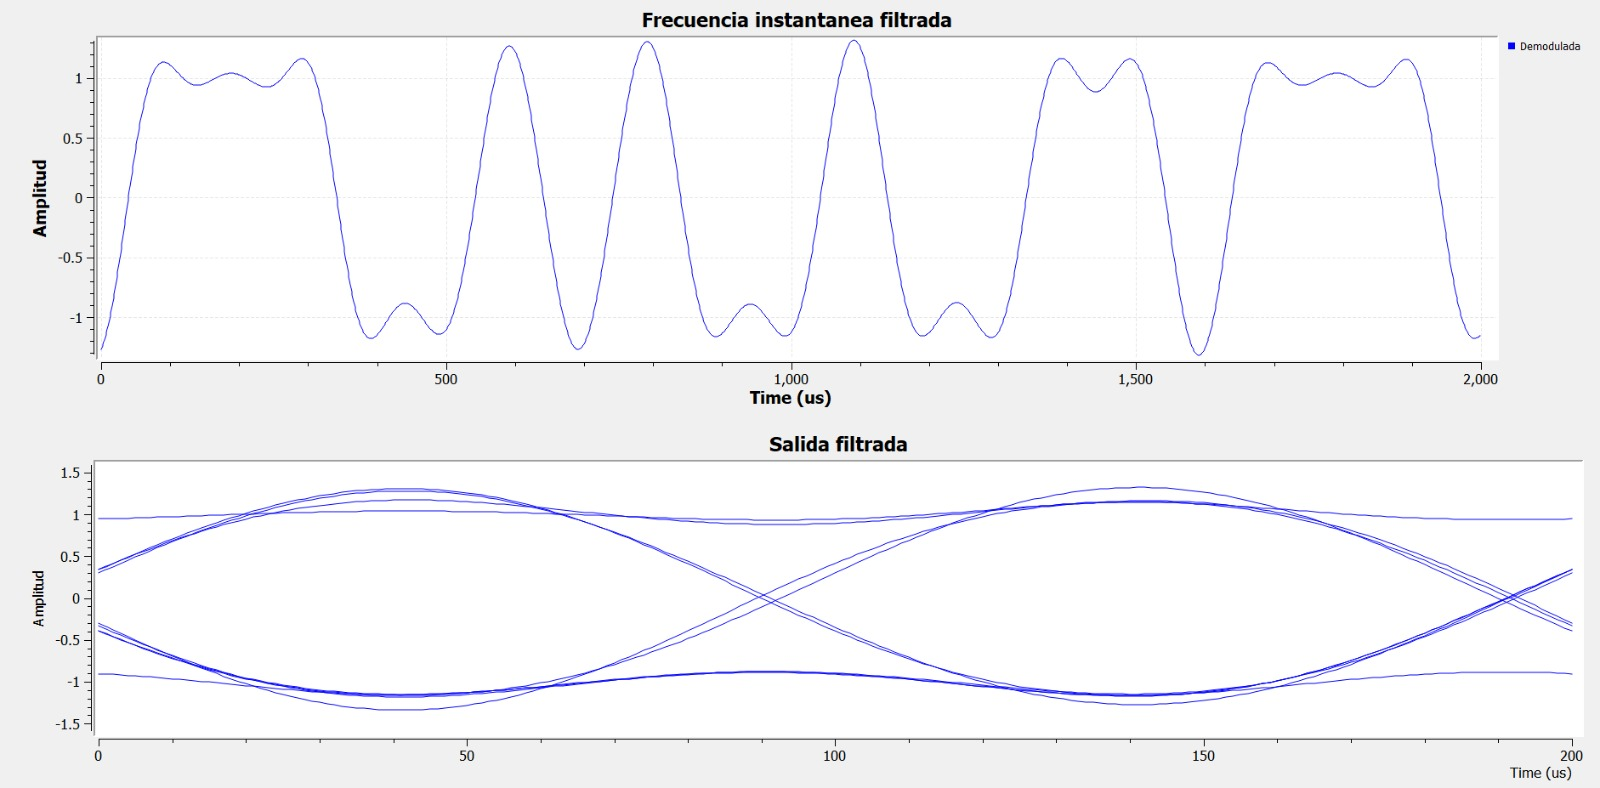
\includegraphics[width=\columnwidth]{p1_rx2.jpeg}\\[2pt]
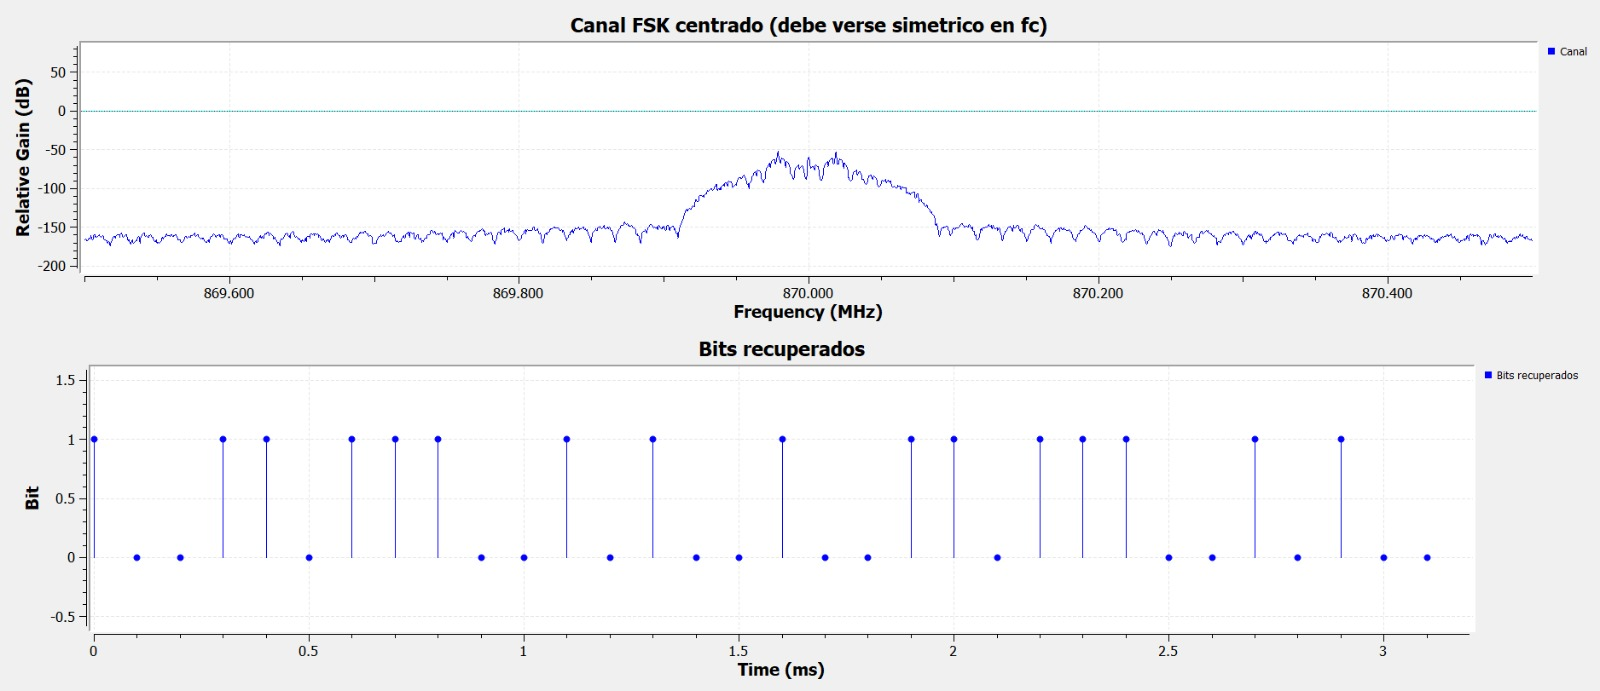
\includegraphics[width=\columnwidth]{p1_rx3.jpeg}
\caption{Prueba 1, receptor: espectro recibido y plano I-Q; frecuencia instantánea filtrada y diagrama de ojo; canal FSK centrado y bits recuperados.}
\label{fig:p1rx}
\end{figure}

\subsection{Prueba 2: transmisión con AWGN ($\sigma = 0.6$)}

Con ruido (Fig.~\ref{fig:p2tx}), el piso del espectro transmitido sube de unos $-100$~dB a unos $-60$~dB relativos, y la envolvente a la entrada del DAC fluctúa alrededor de 0.25 con picos de 0.65, sin llegar a 1. La reducción del nivel de la señal útil se debe al factor $\text{norm} = 1/(1+3\cdot 0.6) = 0.357$ ($-8.9$~dB).

\begin{figure}[!t]
\centering
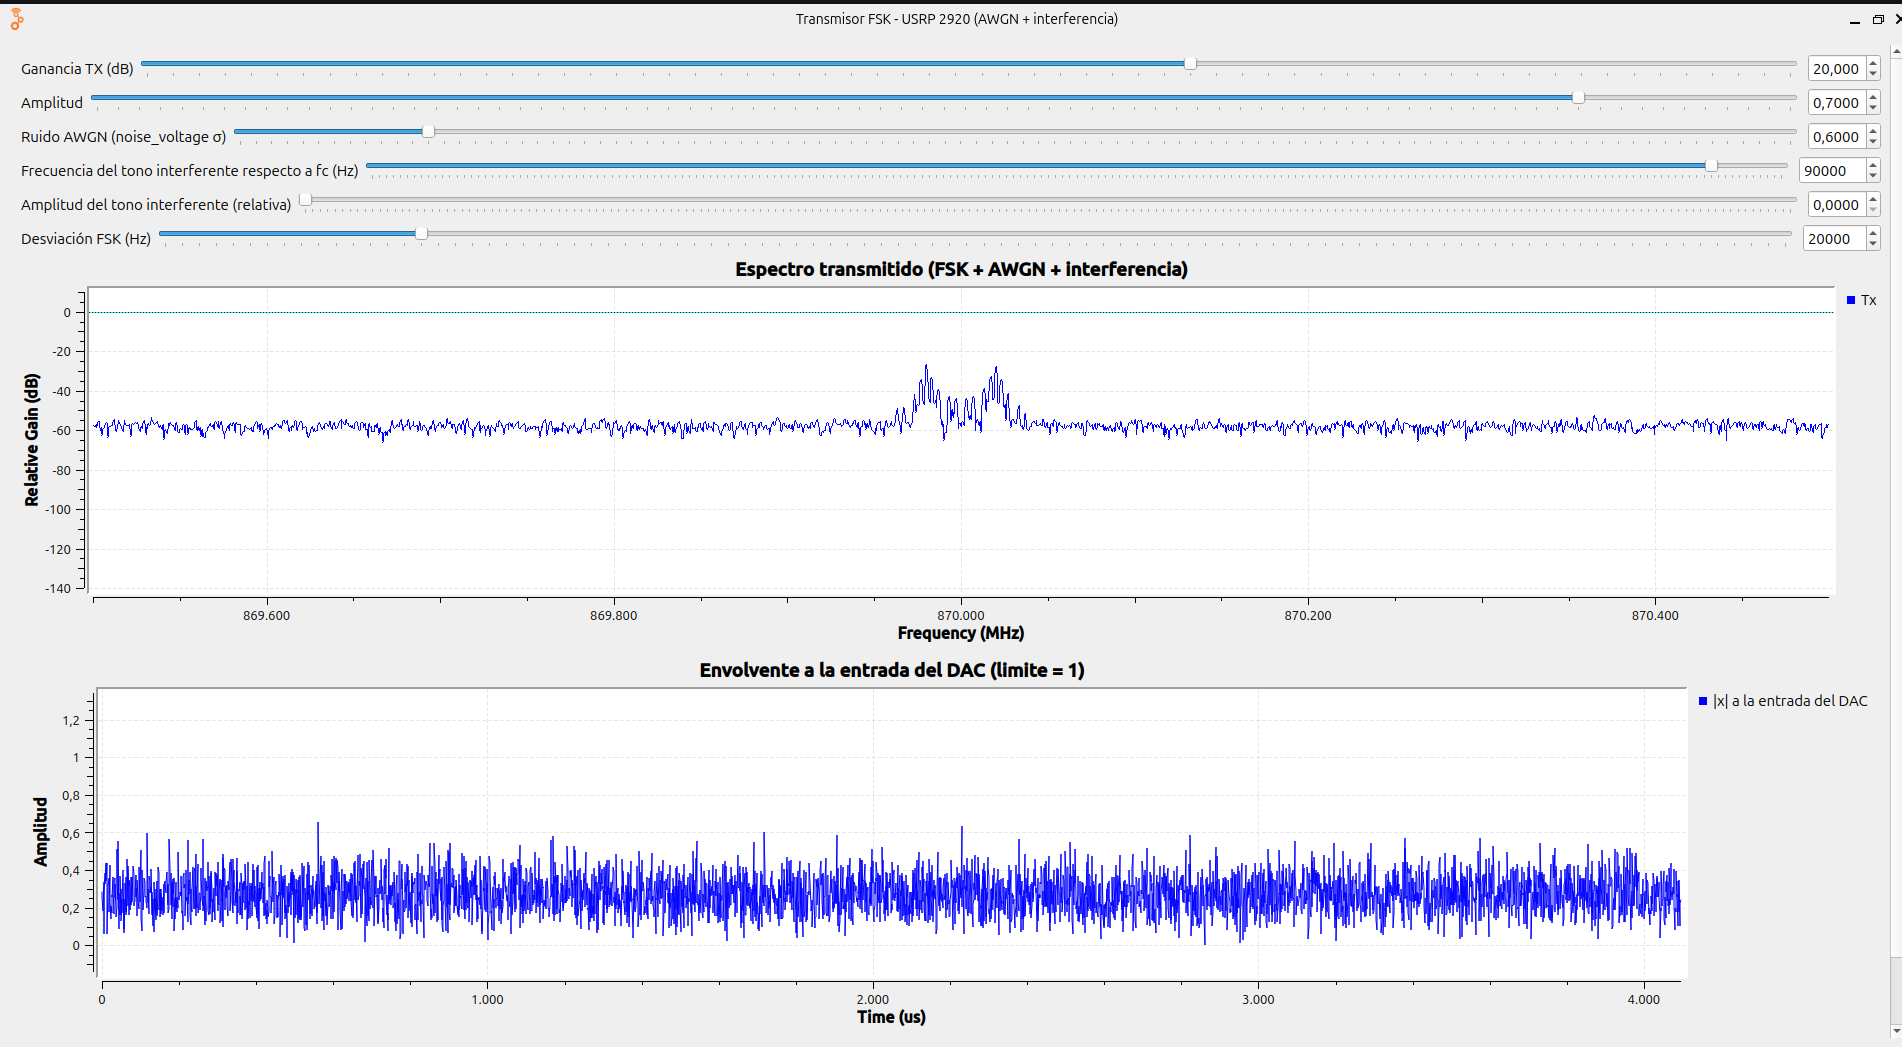
\includegraphics[width=\columnwidth]{p2_tx.png}
\caption{Prueba 2, transmisor: espectro transmitido con AWGN y envolvente a la entrada del DAC ($\sigma = 0.6$, $A = 0$).}
\label{fig:p2tx}
\end{figure}

El analizador (Fig.~\ref{fig:p2an}) mide los tonos en $-57.54$~dBm, unos 12~dB por debajo de la Prueba~1, con la misma separación de 40.801~kHz. El piso sube a cerca de $-80$~dBm en todo el span de 1~MHz, porque el ruido se genera digitalmente a 1~MS/s y ocupa toda la banda de la señal del USRP.

\begin{figure}[!t]
\centering
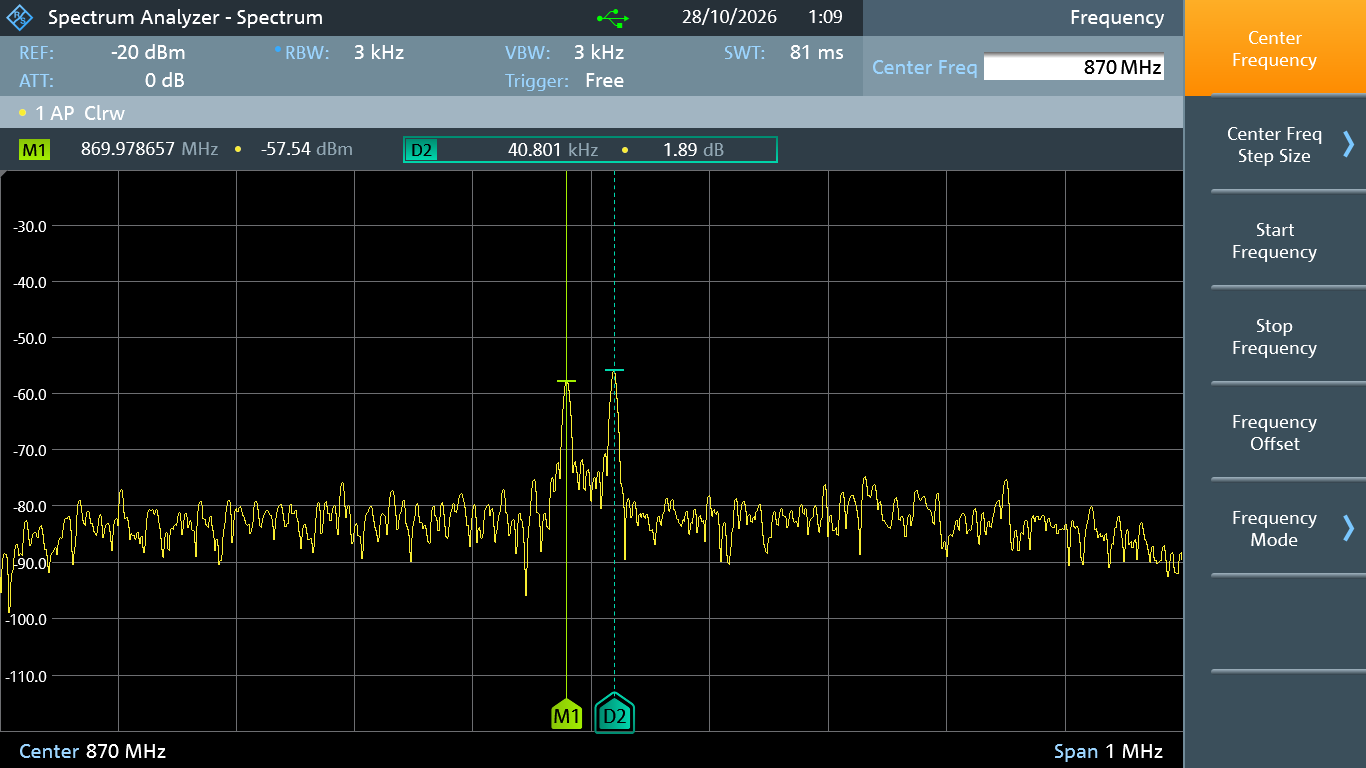
\includegraphics[width=\columnwidth]{p2_analizador.png}
\caption{Prueba 2, analizador de espectro: tonos en $-57.54$~dBm y piso de ruido elevado por el AWGN inyectado.}
\label{fig:p2an}
\end{figure}

En el receptor (Fig.~\ref{fig:p2rx}) el AWGN aparece como una meseta de aproximadamente 1~MHz de ancho (869.5--870.5~MHz) alrededor de los tonos. Este ancho coincide con la tasa de muestreo del transmisor, lo que confirma que el ruido llegó a través del enlace y no se generó en el receptor. El anillo del plano I-Q se engrosa y su radio se reduce, de manera consistente con el escalado \textit{norm}. Aun así, el filtro de canal elimina la mayor parte del ruido fuera de banda: la frecuencia instantánea conserva los dos niveles, el ojo sigue abierto y la secuencia recuperada es la misma que en la Prueba~1, sin errores visibles. Esto es coherente con la simulación de la Fase~2, en la que la BER fue nula para $\sigma \leq 1.5$.

\begin{figure}[!t]
\centering
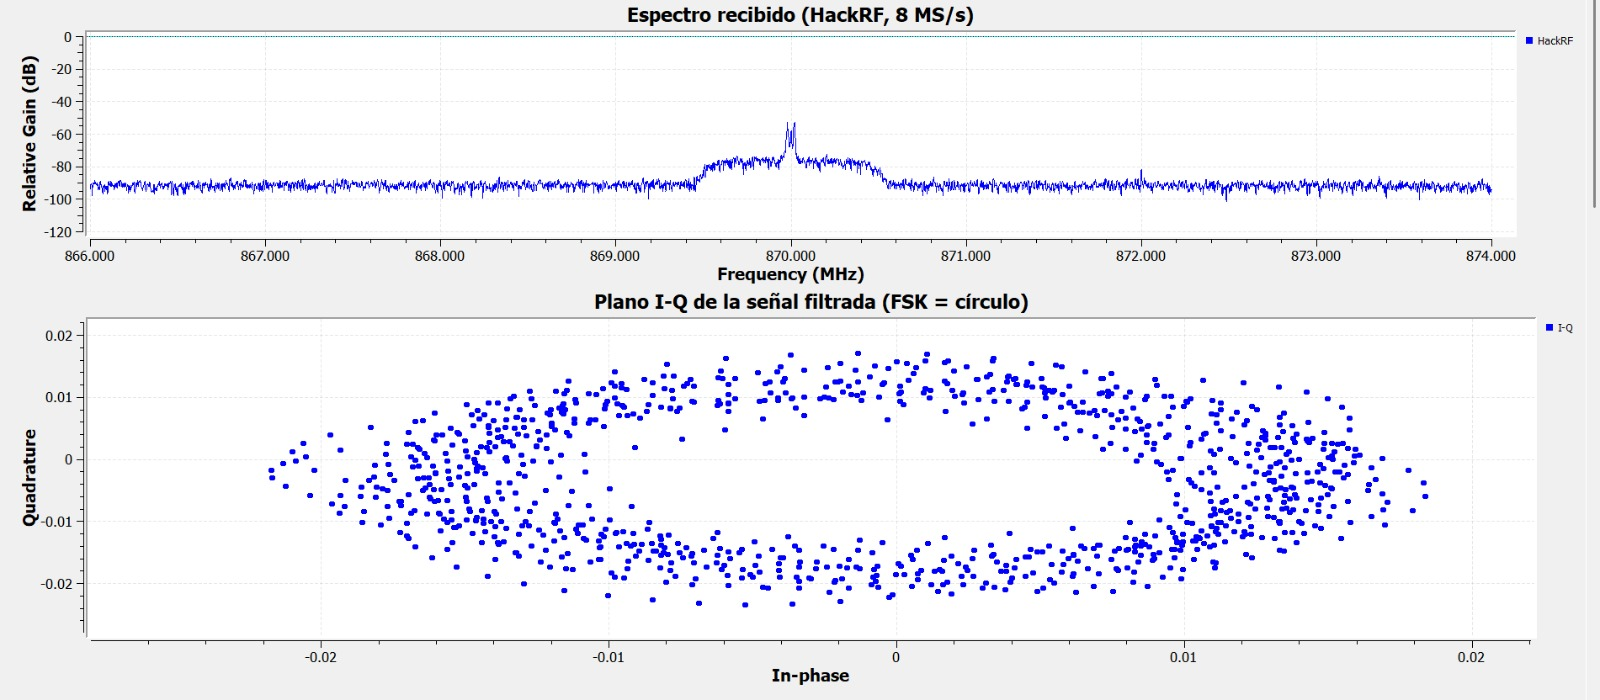
\includegraphics[width=\columnwidth]{p2_rx1.jpeg}\\[2pt]
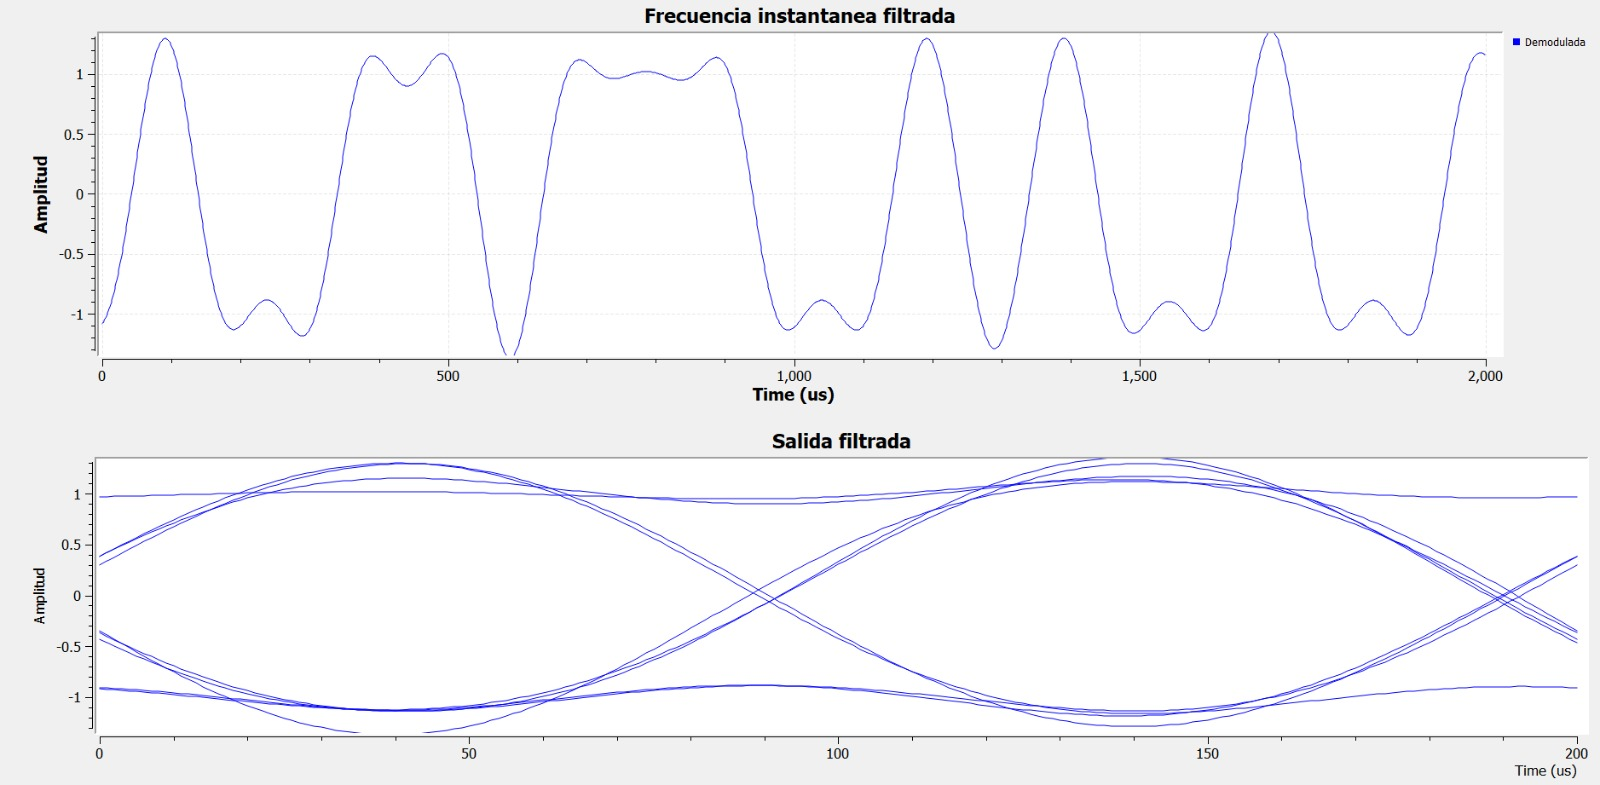
\includegraphics[width=\columnwidth]{p2_rx2.jpeg}\\[2pt]
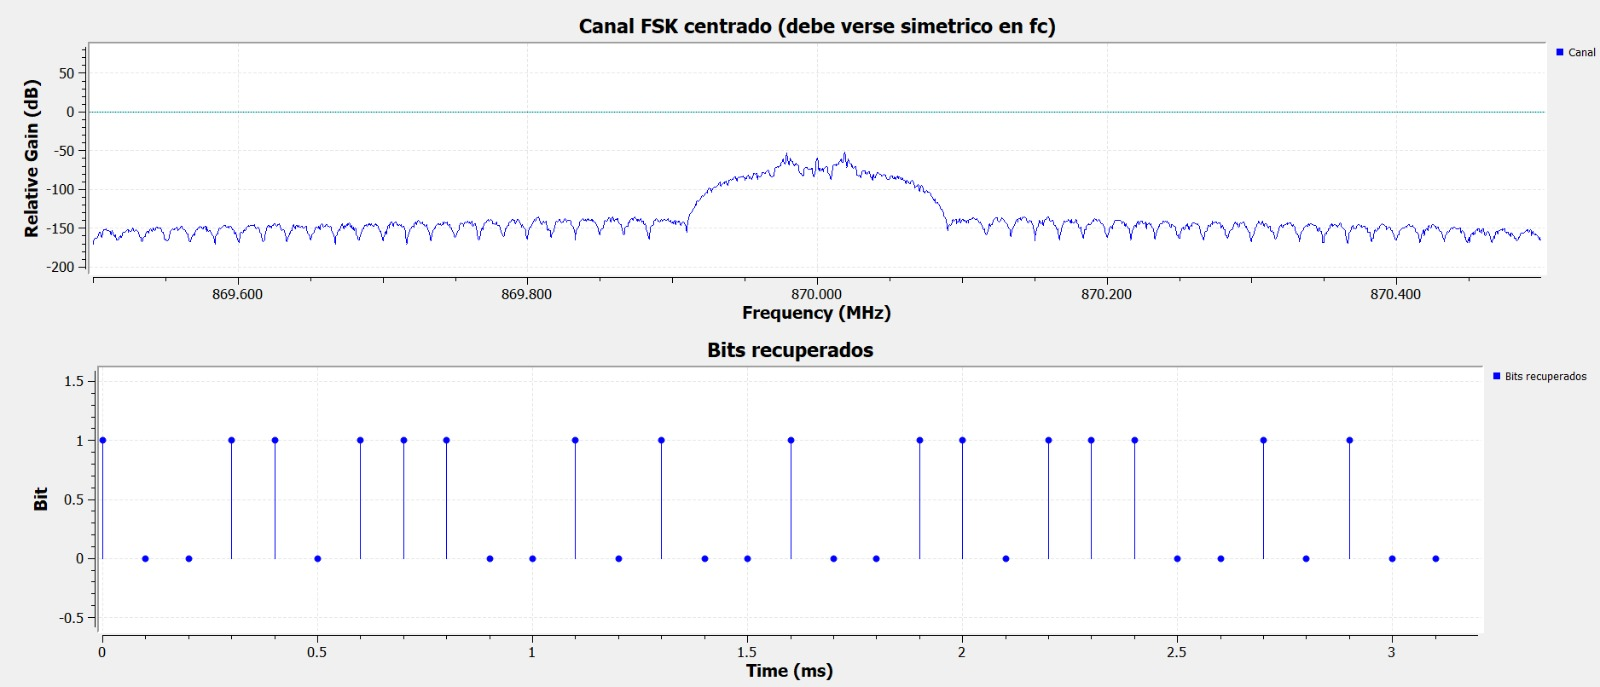
\includegraphics[width=\columnwidth]{p2_rx3.jpeg}
\caption{Prueba 2, receptor: espectro recibido con la meseta de AWGN y plano I-Q engrosado; frecuencia instantánea y diagrama de ojo; canal FSK centrado y bits recuperados.}
\label{fig:p2rx}
\end{figure}

\subsection{Resumen de mediciones}

El Cuadro~\ref{tab:med} compara las dos pruebas.

\begin{table}[!t]
\centering
\caption{Comparación de las pruebas por aire.}
\label{tab:med}
\begin{tabular}{lcc}
\toprule
Medida & Prueba 1 & Prueba 2 \\
\midrule
$\sigma$ inyectado & 0 & 0.6 \\
$E_b/N_0$ en el Tx & $\infty$ & 24.4~dB \\
Nivel de tono (analizador) & $-45.18$~dBm & $-57.54$~dBm \\
Separación entre tonos & 40.801~kHz & 40.801~kHz \\
Piso (analizador, RBW 3~kHz) & $\approx -105$~dBm & $\approx -80$~dBm \\
Radio del anillo I-Q & $\approx 0.035$ & $\approx 0.017$ \\
Ojo & abierto & abierto \\
Bits recuperados & patrón correcto & patrón correcto \\
\bottomrule
\end{tabular}
\end{table}

\section{Errores y problemas encontrados}

El Cuadro~\ref{tab:err} reúne los errores de GNU Radio, UHD y gr-osmosdr y los problemas de hardware que no existían en simulación, junto con su solución.

\begin{table*}[!t]
\centering
\caption{Errores, advertencias y problemas encontrados durante la implementación.}
\label{tab:err}
\begin{tabular}{>{\raggedright}p{4.2cm}>{\raggedright}p{6.2cm}p{6.2cm}}
\toprule
Problema & Causa & Solución \\
\midrule
El transmisor se cerraba al iniciar. & El USRP Sink tenía Sync = \texttt{gps\_time} y llamaba a \texttt{get\_mboard\_sensor("gps\_time")}; el 2920 no tiene GPSDO. & Sync = \texttt{none} (No Sync). \\
Desviación de $\approx 250$~kHz y 125~kbaud en lugar de 20~kHz y 10~kbaud. & El modulador usaba 1~MS/s para calcular la sensibilidad y el USRP transmitía a 12.5~MS/s. & Una sola tasa de 1~MS/s para el modulador y el USRP. \\
Valores de ganancia rechazados. & El control de ganancia iba de $-10$ a 10~dB. & Rango de 0 a 31.5~dB, el de la WBX. \\
Riesgo de saturar el DAC. & Señal de amplitud 1.0 (y mayor al sumar ruido y tono). & \texttt{tx\_amp} = 0.7 y normalización $1/(1+3\sigma+A)$. \\
\texttt{uhd\_find\_devices}: ``No UHD Devices Found''. & El PC no tenía conexión Ethernet con el USRP. & Ejecutar el transmisor en el PC conectado al USRP. \\
Soapy HackRF Source no funcionaba. & Faltaban librerías de SoapySDR en el PC del receptor. & Uso de osmocom Source (gr-osmosdr). \\
Pico de DC del HackRF sobre la señal. & Fuga del oscilador local en el receptor de conversión directa. & Sintonizar en $f_c - \texttt{lo\_offset}$ y recentrar con el Xlating FIR; DC Blocker tras el demodulador. \\
Canal descentrado y lóbulos asimétricos. & Error de frecuencia entre los cristales del USRP y del HackRF. & Control \texttt{freq\_corr} ($\pm 40$~kHz) en el Xlating FIR. \\
Saturación del receptor. & Radios a pocos metros. & AMP apagado y ganancias bajas en Tx y Rx. \\
El bloque Delay no desplazaba la cantidad exacta. & Comportamiento de GNU Radio 3.10.12 al cambiar el retardo. & Ajuste en ejecución con \texttt{sample\_delay}, observando el ojo. \\
Algunos USRP 2920 del aula no transmitían. & Equipos en malas condiciones por el uso. & Cambio a un USRP 2920 en buen estado. \\
Señal débil o intermitente en Tx/Rx. & Conectores de antena (puertos TX/RX) flojos o mal acoplados. & Ajuste y apriete de los acoples de las antenas. \\
\bottomrule
\end{tabular}
\end{table*}

\section{Preguntas de investigación}

\textit{1) ¿Por qué el Channel Model ya no representa el canal cuando se conecta un SDR real?} Porque la señal sale al aire como RF real. El canal pasa a ser físico: pérdida por distancia, multitrayecto del laboratorio, ruido térmico de los receptores, interferencias reales e imperfecciones de los radios (offset de frecuencia, DC, ruido de fase)~\cite{proakis}. Un bloque de canal solo sirve para \emph{agregar} degradación controlada, como el AWGN inyectado en la Prueba~2, pero ya no representa el medio.

\textit{2) ¿Por qué un hardware Sink/Source hace innecesario el Throttle?} Porque el reloj del conversor (DAC del USRP o ADC del HackRF) consume o entrega exactamente \textit{radio\_rate} muestras por segundo y bloquea el flujo al ritmo real. Un Throttle añadiría un segundo reloj por software, impreciso, que compite con el del radio y provoca underflows u overflows.

\textit{3) ¿Qué diferencia existe entre la frecuencia central RF y las frecuencias de la señal en banda base?} La señal en banda base es compleja y está centrada en 0~Hz: la FSK ocupa $\pm 20$~kHz ($\pm 30$~kHz por Carson). El radio la traslada a $f_c = 870$~MHz, de modo que el bit 1 sale en 870.02~MHz y el bit 0 en 869.98~MHz. En el receptor, la señal vuelve a banda base desplazada \texttt{lo\_offset} y el Xlating FIR la recentra en 0~Hz.

\textit{4) ¿Qué ocurre si el transmisor genera muestras más lentamente que la tasa exigida por el SDR?} El buffer del USRP se vacía y se produce un underflow (``U'' en consola). El radio transmite huecos o ceros, la señal sale entrecortada, se pierden símbolos y aparecen transitorios espectrales.

\textit{5) ¿Qué diferencia hay entre aumentar la amplitud digital antes del Sink y aumentar la ganancia RF?} La amplitud digital escala las muestras antes del DAC; si $|x| > 1$ el DAC recorta, lo que genera distorsión y espurias. La ganancia RF amplifica la señal analógica después del DAC sin cambiar su forma digital; su límite es la linealidad del amplificador y no saturar el receptor cercano. Lo correcto es usar una amplitud digital alta sin recortar (0.7 en este caso) y ajustar el nivel con la ganancia RF.

\textit{6) ¿Qué limita la tasa de muestreo útil?} Todos los factores: el conversor (reloj maestro de 100~MHz en el 2920 y hasta 20~MS/s en el HackRF), la interfaz (Gigabit Ethernet, unos 25~MS/s a 16~bits, y USB~2.0, unos 20~MS/s a 8~bits) y el procesamiento, porque la CPU debe ejecutar el flujograma en tiempo real. Las tasas usadas (1 y 8~MS/s) están muy por debajo de esos límites.

\textit{7) ¿Por qué dos radios sintonizados al mismo valor pueden presentar un offset de frecuencia?} Cada radio genera su portadora a partir de su propio oscilador de cristal, con una tolerancia de algunos ppm. Con $\pm 10$~ppm a 870~MHz la diferencia puede ser de varios kHz. Los radios no comparten una referencia común de 10~MHz/PPS y la temperatura también influye. Por eso el receptor incluye \texttt{freq\_corr}.

\textit{8) ¿Qué parámetros se conservan del diseño simulado y cuáles aparecen solo con hardware?} Se conservan $R_s = 10$~kbaud, $\Delta f = 20$~kHz, $h = 4$, $sps = 100$, $bb\_rate = 1$~MS/s, el mapeo NRZ y el discriminador. Solo con hardware aparecen $f_c$, las ganancias (TX, AMP, LNA, VGA), el puerto de antena, la dirección del dispositivo, la tasa del radio (8~MS/s), la decimación por 8, \texttt{lo\_offset}, \texttt{freq\_corr}, el sincronismo, el ancho de banda del filtro analógico y el Bias-T.

\textit{9) ¿Qué riesgo existe al conectar directamente dos radios por coaxial sin atenuación?} El USRP puede entregar del orden de $+15$ a $+20$~dBm y la entrada del HackRF tolera como máximo unos $-5$~dBm. Sin atenuación se satura el receptor y, en el peor caso, se daña su LNA de forma permanente. Por eso las pruebas conducidas exigen atenuadores (por ejemplo de 30 a 60~dB). En este trabajo se transmitió por aire, a unos 3~m y con ganancias bajas.

\textit{10) ¿Qué evidencia demostraría que el problema está en la configuración RF y no en la modulación digital?} La simulación con los mismos parámetros funciona con BER nula. Si en hardware el espectro aparece desplazado, asimétrico, saturado, con el pico de DC encima o con un nivel muy bajo, el problema es de RF. La prueba concreta es comparar en el analizador y en el espectro recibido la forma de la FSK (dos lóbulos separados 40~kHz) con la PSD simulada: si coinciden y, al corregir \texttt{freq\_corr} o las ganancias, se recupera la onda cuadrada de la frecuencia instantánea, la modulación digital está bien. Es lo que se observó en las dos pruebas.

\section{Análisis}

Las mediciones confirman que el enlace físico reproduce el diseño. La separación de 40.8~kHz medida en el analizador corresponde a $2\Delta f$ y es igual en ambas pruebas, de modo que la sensibilidad del modulador y la tasa de 1~MS/s llegaron intactas al aire. La diferencia de unos 12~dB en el nivel de los tonos entre las pruebas se explica principalmente por la normalización ($-8.9$~dB), que reparte la amplitud disponible del DAC entre la señal y el ruido.

La Prueba~2 muestra además el papel del filtro de canal: el ruido inyectado ocupa 1~MHz, pero el Xlating FIR deja pasar solo unos $\pm 100$~kHz alrededor de la señal, así que el discriminador trabaja con un $E_b/N_0$ alto (24.4~dB en el transmisor) y no aparece el efecto umbral observado en la simulación sin filtro. Por eso la secuencia se recupera sin errores visibles en ambas pruebas.

El Cuadro~\ref{tab:sep} responde a la conclusión técnica que pide la guía: qué parámetros pertenecen al diseño de comunicaciones y cuáles a la interfaz de hardware.

\begin{table}[!t]
\centering
\caption{Parámetros de diseño frente a parámetros de hardware.}
\label{tab:sep}
\begin{tabular}{>{\raggedright}p{3.6cm}p{3.9cm}}
\toprule
Diseño de comunicaciones & Interfaz de hardware \\
\midrule
$R_s = 10$~kbaud & $f_c = 870$~MHz \\
$\Delta f = 20$~kHz, $h = 4$ & Ganancias TX, AMP, LNA, VGA \\
$sps = 100$, $bb\_rate = 1$~MS/s & radio\_rate (1 y 8~MS/s), decimación $\times 8$ \\
Mapeo NRZ, discriminador & Device Address/Arguments, antena \\
Filtro de canal, integración y umbral & \texttt{lo\_offset}, \texttt{freq\_corr}, DC Blocker \\
Amplitud y normalización frente al ruido & Sync, Clock/Time Source, Bias-T, Bandwidth \\
\bottomrule
\end{tabular}
\end{table}

\section{Conclusiones}

Se implementó el enlace BFSK de telemetría industrial sobre hardware SDR real, transmitiendo con un USRP 2920 y recibiendo con un HackRF One a 870~MHz, sin modificar los parámetros de diseño de la aplicación: $R_s = 10$~kbaud, $\Delta f = 20$~kHz y $sps = 100$.

La principal diferencia frente a la simulación fue la adaptación de tasas: el USRP aceptó directamente la tasa de banda base de 1~MS/s, mientras que el HackRF requirió 8~MS/s y una decimación por 8 en el receptor. También aparecieron problemas que no existían en simulación, como el sincronismo GPS inexistente, el pico de DC, el offset de frecuencia entre cristales y el riesgo de saturación, que se resolvieron con parámetros propios de la interfaz de hardware.

En las dos pruebas por aire el analizador midió una separación entre tonos de 40.8~kHz, coherente con la desviación diseñada, y el receptor recuperó el patrón transmitido sin errores visibles, incluso con AWGN inyectado de $\sigma = 0.6$. Como trabajo futuro queda transmitir mensajes con preámbulo y palabra de sincronización, y medir la BER en hardware.

\begin{thebibliography}{9}

\bibitem{guia1} Universidad Industrial de Santander, ``Proyecto Final de Comunicaciones II -- Fase 2: Modelado y Simulación (Guía 1)'', Guía de laboratorio.

\bibitem{guia2} Universidad Industrial de Santander, ``Proyecto Final de Comunicaciones II -- Diseño del Sistema Tx--Canal--Rx en GNU Radio (Guía 2)'', Guía de laboratorio.

\bibitem{guia3} O. Tíjaro y R. Zamora, ``Proyecto Final de Comunicaciones II -- Fase 3: Configuración inicial de HackRF One y USRP en GNU Radio (Guía 3)'', Universidad Industrial de Santander.

\bibitem{hackrf} Great Scott Gadgets, ``HackRF One'', disponible en: \url{https://hackrf.readthedocs.io/en/stable/hackrf_one.html}.

\bibitem{osmosdr} Osmocom, ``gr-osmosdr'', disponible en: \url{https://osmocom.org/projects/gr-osmosdr/wiki}.

\bibitem{uhdsink} GNU Radio Project, ``USRP Sink'', disponible en: \url{https://wiki.gnuradio.org/index.php/USRP_Sink}.

\bibitem{uhd} Ettus Research, ``UHD Manual'', disponible en: \url{https://files.ettus.com/manual/}.

\bibitem{proakis} J. G. Proakis y M. Salehi, \textit{Digital Communications}, 5th ed., McGraw-Hill, 2008.

\end{thebibliography}

\end{document}
